\chapter{Implementation}\label{ch:impl}

The implementation combines a Rust cryptographic core and directory with a TypeScript verifier
embedded in Signal Desktop. This chapter covers their architecture, integration, parity testing,
engineering constraints, and reproducibility.

% ============================================================================
\section{Architecture and Language Boundary}\label{sec:impl-strategy}

The implementation separates a measured Rust reference system from a TypeScript verifier embedded in
Signal Desktop. The standalone \texttt{duet} crate contains the directory, cryptographic operations,
auditor, and benchmarks. Rust was chosen because comparable systems use it and because the crate can
be measured without Signal or libsignal dependencies~\cite{malvai2023parakeet,facebook-akd}.
\Cref{fig:impl-overview} shows this language and trust boundary.

The TypeScript layer implements the client-side proof checks and user-interface path. It verifies
prefix, log, VRF, and signed-head evidence locally, performs the required raw-label writes, and is
checked against Rust through fixed vectors and live wire-parity tests. The formats follow the IETF
KeyTrans design, but no Go interoperability is claimed because Signal and DUET deliberately use
different prefix-proof encodings~\cite{ietf-keytrans-protocol,signal-kt-server}.

The Rust service is an in-memory, single-machine prototype. The Signal integration uses a deterministic
conversation-secret stand-in and a seeded Double Ratchet simulation. These exercise the construction and wire format but do not
demonstrate secrecy-dependent label unpredictability or real-ratchet security. The identity-key path
itself is not simulated, because the verifier is invoked at Signal Desktop's real peer-key-retrieval
boundary. Production integration must obtain the live conversation secret and ratchet state from libsignal
(\cref{ch:discussion}).

\begin{figure}[t]
\centering
% fig-impl-overview.tex — implementation and process boundaries (horizontal row).
% Three role/process boxes of equal fixed height; functions on separate lines.
% Label: \label{fig:impl-overview}
\hyphenpenalty=10000\exhyphenpenalty=10000
\resizebox{\linewidth}{!}{%
\begin{tikzpicture}[>=Stealth,font=\scriptsize,
   box/.style={draw,rounded corners,align=center,inner sep=5pt,minimum height=34mm}]
  \node[box,fill=black!4,text width=4.4cm] (cli) at (0,0)
    {\textbf{Signal Desktop client component}\\[1pt]{\scriptsize integrated TypeScript}\\[6pt]{\scriptsize proof verifier}\\{\scriptsize background monitor}\\{\scriptsize lifecycle hooks}\\{\scriptsize warning interface}};
  \node[box,fill=black!6,text width=5.4cm] (srv) at (7.4,0)
    {\textbf{DUET directory server and cryptographic core}\\[1pt]{\scriptsize \texttt{duet} crate, Rust}\\[6pt]{\scriptsize sparse Merkle prefix tree}\\{\scriptsize append-only Merkle log}\\{\scriptsize signed heads}\\{\scriptsize dual-index and CEA operations}\\{\scriptsize HTTP API}};
  \node[box,fill=black!4,text width=4.4cm] (aud) at (15.8,0)
    {\textbf{Auditor process}\\[1pt]{\scriptsize \texttt{duet} crate, Rust}\\[6pt]{\scriptsize verify signed heads and}\\{\scriptsize consistency proofs}\\{\scriptsize replay declared transitions}\\{\scriptsize compare primary and}\\{\scriptsize staged views}};
  \draw[<->] (cli.east) -- node[above=3pt,font=\scriptsize,fill=white,inner sep=1pt]{HTTP/JSON} (srv.west);
  \draw[<->,dashed] (srv.east) -- node[above=3pt,align=center,font=\scriptsize,fill=white,inner sep=1pt]{signed heads, epoch\\deltas, consistency proofs} (aud.west);
\end{tikzpicture}%
}

\caption[Implemented architecture.]{The TypeScript verifier checks responses from the Rust directory
server, while an independent auditor obtains signed heads and epoch disclosures from a separate
vantage.}
\label{fig:impl-overview}
\end{figure}

% ============================================================================
\section{The Rust Cryptographic Core}\label{sec:impl-modules}

The \texttt{duet} crate implements a path-compressed sparse Merkle directory, an RFC~9162 append-only
log, ECVRF-EDWARDS25519-SHA512-TAI, signed tree heads, dual-index and CEA constructions, an HTTP
server, and an independent auditor~\cite{rfc9162,rfc9381,dowling2023acka}. The crates \texttt{sha2},
\texttt{hkdf}, \texttt{ed25519-dalek}, and \texttt{curve25519-dalek} supply the standard primitives, so
the ECVRF is the one primitive written by hand, and it is checked against the RFC~9381 vectors.
\Cref{fig:impl-modules} shows the module structure, and \cref{tab:impl-modules} records the inventory
with its specification grounding and conformance evidence.

\begin{figure}[ht]
\centering
% fig-impl-modules.tex — directory core with external client component and auditor.
% The server core (KTServer) composes the prefix tree, Merkle log, ECVRF, and the
% Ed25519 signer; the prefix tree, Merkle log, and KTServer itself hash through the
% shared SHA-256 component. The client component and the auditor are separate
% processes that reach the directory over the HTTP interface.
% Label: \label{fig:impl-modules}
\resizebox{\textwidth}{!}{%
\begin{tikzpicture}[>=Stealth,font=\scriptsize,
   cmp/.style={draw,rounded corners,align=center,minimum height=8mm,inner sep=3pt,fill=white},
   ext/.style={draw,rounded corners,align=center,minimum height=10mm,inner sep=3pt,fill=black!5},
   band/.style={font={\footnotesize\itshape},anchor=east,text=black!70}]

  % ---- server stack (left/centre) ----
  \node[cmp,minimum width=5.0cm] (api) at (0,5.3) {\textbf{HTTP server}\\lookup, update, and consistency API};
  \node[cmp,minimum width=3.0cm] (dir) at (0,3.8) {\textbf{Directory service}\\(\texttt{KTServer})};
  \node[cmp,minimum width=2.3cm] (ptree) at (-3.6,2.1) {Sparse Merkle\\prefix tree};
  \node[cmp,minimum width=2.1cm] (mlog)  at (-1.2,2.1) {Append-only\\Merkle log};
  \node[cmp,minimum width=1.9cm] (vrf)   at ( 1.0,2.1) {ECVRF};
  \node[cmp,minimum width=2.3cm] (sig)   at ( 3.3,2.1) {Ed25519\\signer};
  \node[cmp,minimum width=8.0cm] (hash)  at (-0.15,0.5) {SHA-256 hashing};
  % bands
  \node[band] at (-5.2,5.3) {API};
  \node[band] at (-5.2,3.8) {server core};
  \node[band,align=right] at (-5.2,2.1) {authenticated\\structures};
  \node[band] at (-5.2,0.5) {hashing layer};
  % server dependency edges
  \draw[->] (api) -- (dir);
  \foreach \n in {ptree,mlog,vrf,sig}{\draw[->] (dir) -- (\n);}
  \foreach \n in {ptree,mlog}{\draw[->] (\n) -- (\n |- hash.north);}
  \draw[->] (dir.south) -- (hash.north);

  % ---- external client component ----
  \node[ext,minimum width=3.0cm,text width=2.8cm] (cli) at (7.2,5.3) {\textbf{Client component}\\Signal Desktop};
  \draw[<->] (cli.west) -- node[above,font=\scriptsize,fill=white,inner sep=1pt]{HTTP/JSON} (api.east);

  % ---- auditor (separate process) ----
  \node[ext,minimum width=3.2cm,text width=3.0cm] (aud) at (7.2,2.9) {\textbf{Auditor}\\transition replay and head comparison};
  \draw[<->,dashed] (aud.west) -- node[above,align=center,font=\scriptsize,fill=white,inner sep=1pt,pos=0.5]{signed heads,\\consistency proofs,\\and epoch deltas} (api.east);
\end{tikzpicture}%
}

\caption[Module structure of the \texttt{duet} crate.]{Module structure of the \texttt{duet} crate.
The directory, log, and VRF modules are consumed by the server, the auditor, and the benchmark
harness alike.}
\label{fig:impl-modules}
\end{figure}

\begin{table}[ht]
\centering
\caption{The \texttt{duet} crate's modules and their specification grounding.}
\label{tab:impl-modules}
\setlength{\extrarowheight}{2pt}
\footnotesize
\begin{tabular}{@{}p{3.0cm}p{5.0cm}p{4.4cm}@{}}
\toprule
Module & Specification implemented & Conformance evidence \\
\midrule
\texttt{hashing} & RFC~6962 Section~2.1 leaf/node domain tags~\cite{rfc6962} & domain-separation unit tests \\
\texttt{merkle\_log} & RFC~9162 Sections~2.1.3 and~2.1.4 inclusion and consistency verifiers~\cite{rfc9162} & exhaustive inclusion + every $(m,n)$ consistency pair up to size 64, plus forgery rejection \\
\texttt{prefix\_tree} & IETF KeyTrans sparse Merkle tree, path-compressed~\cite{ietf-keytrans-protocol} & client-side root recompute from compressed proof \\
\texttt{vrf} & RFC~9381 ECVRF-EDWARDS25519-SHA512-TAI, suite \texttt{0x03}~\cite{rfc9381} & RFC~9381 App.~B.3 test vectors \\
\texttt{dual\_index} & RFC~5869 HKDF-SHA256 label derivation~\cite{rfc5869} with warning-payload MAC (\cref{alg:dualindex}) & label derivation by cross-implementation vectors vs.\ TypeScript, MAC by cross-implementation sealed-payload vector vs.\ TypeScript plus roundtrip + injection-rejection unit tests, wired into both clients' warning write/read paths \\
\texttt{server} & KeyTrans combined-tree semantics + Ed25519 STH~\cite{ietf-keytrans-protocol} with write-once raw-label policy + per-epoch declared update set (\cref{alg:server}) & STH signature happy/tamper/wrong-key, committed-snapshot search, write-once rejection, delta records inserts and rotations \\
\texttt{auditor} & cross-vantage fork detection + per-epoch transition audit (\cref{alg:auditor}) & append-only audit + equivocation tests, and transition audit catches undeclared deletion and modification \\
\texttt{monitor} & writer-side persistence check + deletion-evidence bundle (\cref{alg:detect}) & persistence holds while committed, and deletion yields evidence that verifies against the server's signed heads \\
\texttt{cea} & ACKA example CEA construction~\cite{dowling2023acka}, server-composed register/verify with sender pre-post check and advance-only-on-success (\cref{alg:cea}) & cross-implementation vectors vs.\ TypeScript, plus occupied-label and no-advance-on-fork/not-posted tests \\
\texttt{hook\_process\_\allowbreak prekey\_bundle} & documentation-only libsignal integration module, compiled with the crate but not invoked as an executable hook & marks where a production binding of the live X3DH secret could be inserted \\
\bottomrule
\end{tabular}
\end{table}

\FloatBarrier
\subsection{Directory State and Cryptography}\label{ssec:impl-core-state}
\label{ssec:impl-core-crypto}

The directory materializes only populated prefix paths and bitmap-compresses proofs. The walk is a
fixed 256-bit descent, but a compressed leaf terminates it early, and the chain of empty-sibling
hashes below that point is memoized lazily rather than recomputed. A transmitted proof carries about $\lceil \lg N \rceil$ sibling hashes, because the chain of
empty-sibling hashes below a compressed leaf is elided rather than sent. Update cost is a separate
property. With the trie depth fixed at $d=256$, copying the affected paths for $k$ modified labels
costs $O(kd)$, which is $O(k)$ in $k$ and independent of $N$.

A committed epoch freezes a snapshot, appends its root to the log, and signs the resulting head.
Client recomputation checks each response without trusting the directory operator. Dual-index labels use
HKDF-SHA256, while global identity labels use the RFC ECVRF. The main non-linear implementation cost
is epoch commit, which deep-clones the current tree into the committed snapshot. The full
module and data-structure detail is preserved in \cref{sec:apiref-engineering}.

\subsection{Server, Auditor, and Benchmark Boundary}\label{ssec:impl-core-server}
\label{ssec:impl-bench}

An \texttt{axum} and \texttt{tokio} server holds the directory behind a single
\texttt{Arc<Mutex<KTServer>>} with no sharding, which is adequate for a single-machine prototype and is
one of the constraints \cref{ch:discussion} returns to. The server exposes public lookup and monitoring
operations plus a privileged unchecked-overwrite interface used only by the adversarial harness.
Write-once enforcement returns 409 Conflict when a dual-index, warning, or CEA label is already
occupied, so a replacement is refused rather than silently applied. A separate \texttt{ureq} auditor
binary obtains signed heads from its own vantage.

Every commit publishes a declared set of inserts and rotations at an epoch-delta endpoint, and each
rotation discloses its prior value. \Cref{fig:impl-transition-audit} shows the resulting audit. The
auditor applies the declared set to a candidate replica and accepts only if the recomputed root equals
the committed root, which mirrors the \texttt{AuditorUpdate} role in the IETF architecture. Deletion is
not expressible in the delta format, so an omitted warning or an immutable-slot replacement makes the
roots diverge and is reported rather than absorbed. A tested writer-side persistence component can
additionally combine an original inclusion proof, a later non-inclusion proof, and consistency between
the two signed heads into independently verifiable deletion evidence, but it is not yet wired into the
live monitor. Initial ownership of an empty raw label is not authenticated, so a malicious client can
still occupy an unclaimed slot first.

\begin{figure}[htbp]
\centering
% fig-impl-transition-audit.tex — the transition auditor's state flow (Alg 7).
% After head classification the auditor verifies the append-only consistency
% proof for a GROWN head (classify_head -> GrewNeedsConsistency in kt_auditor.rs)
% and fails closed on a missing/invalid proof, BEFORE any delta replay.
% Label: \label{fig:impl-transition-audit}
\begin{tikzpicture}[>=Stealth,font=\scriptsize,node distance=5.0mm,
  proc/.style={draw,rounded corners,align=center,inner sep=3pt,minimum width=5.6cm,minimum height=7mm},
  dec/.style={draw,align=center,inner sep=3pt,minimum width=5.6cm,minimum height=7mm,fill=blue!6},
  bad/.style={draw,rounded corners,align=center,inner sep=3pt,draw=red!60!black,fill=red!3},
  rtr/.style={draw,rounded corners,align=center,inner sep=3pt,draw=orange!80!black,fill=orange!4},
  note/.style={align=center,font=\tiny\itshape,text=black!55},
  good/.style={draw,rounded corners,align=center,inner sep=3pt,draw=green!50!black,fill=green!4,minimum width=5.6cm}]

  \node[proc] (n1) {receive new head; verify STH signature};
  \node[dec,below=of n1] (n2) {rollback, or equal size with a different root?};
  \node[dec,below=of n2] (nc) {log grew (new size $>$ baseline)?};
  \node[proc,below=of nc] (ncp) {fetch + verify RFC~9162 consistency proof\\(append-only, baseline\,$\to$\,new head)};
  \node[proc,below=of ncp] (n3) {fetch the epoch's declared transition (delta)};
  \node[proc,below=of n3] (n4) {clone the committed mirror into scratch};
  \node[proc,below=of n4] (n5) {replay each Insert / Rotate into scratch\\(A1: reject a duplicate insert; C2: reject an immutable rotation)};
  \node[dec,below=of n5] (n6) {replayed scratch root $=$ committed root?};
  \node[good,below=of n6] (n7) {commit mirror, cursor and head atomically};

  \draw[->] (n1) -- (n2);
  \draw[->] (n2) -- node[left,pos=0.45]{no} (nc);
  \draw[->] (nc) -- node[left,pos=0.45]{yes} (ncp);
  \draw[->] (ncp) -- (n3);
  \draw[->] (n3) -- (n4);
  \draw[->] (n4) -- (n5);
  \draw[->] (n5) -- (n6);
  \draw[->] (n6) -- node[left,pos=0.45]{yes} (n7);

  % failure / retry / no-op branches to the right
  \node[bad,right=10mm of n2] (b2) {reject: raise Fork};
  \draw[->] (n2.east) -- node[above,font=\tiny]{yes} (b2.west);
  \node[rtr,right=10mm of nc] (bnc) {same size $+$ root:\\idempotent, no state change};
  \draw[->] (nc.east) -- node[above,font=\tiny]{no} (bnc.west);
  \node[bad,right=10mm of ncp] (bcp) {missing / malformed / invalid proof:\\ALARM (latch), no replay};
  \draw[->] (ncp.east) -- node[above,font=\tiny]{fail} (bcp.west);
  \node[rtr,right=10mm of n3] (b3) {on fetch failure: discard\\scratch, retry (no fork)};
  \draw[->] (n3.east) -- node[above,font=\tiny]{fail} (b3.west);
  \node[bad,right=10mm of n6] (b6) {ALARM: transition\\audit failed};
  \draw[->] (n6.east) -- node[above,font=\tiny]{no} (b6.west);
\end{tikzpicture}

\caption[Per-epoch transition audit.]{Per-epoch transition audit. The auditor replays the declared
insert and rotation set against its own replica and accepts the epoch only when the recomputed root
equals the committed root.}
\label{fig:impl-transition-audit}
\end{figure}

The benchmark harness invokes the Rust server in process. Its timings therefore measure local
cryptographic work rather than HTTP, Electron, database, or network cost. The measurement environment
is in \cref{sec:bench-env}. The reproduction procedure is in \cref{sec:bench-repro}.
\FloatBarrier

% ============================================================================
\section{Signal Desktop Integration}\label{sec:impl-signal}

The embedded TypeScript client verifies Rust directory responses and reports the result through a
conversation badge and banner. Successful verification produces a green state. An unavailable check
produces an amber notice. A proof failure, key mismatch, or authenticated peer warning produces a red
warning.

\subsection{Client Verification and Lifecycle}\label{ssec:impl-verifier}
\label{ssec:impl-hooks}

Node's cryptographic provider supplies SHA-256, SHA-512, HMAC-SHA256, Ed25519, and X25519, while the
ECVRF arithmetic is implemented in TypeScript. At the peer-key-retrieval boundary, which is Signal
Desktop's own identity-key path and not a simulation, the client performs the complete verification
chain in \cref{ssec:design-verify}. Invalid or absent signed heads, proof failures, and mismatching
keys produce rejecting verification verdicts. The current hook reports the verdict but does not block
session establishment, which is a deliberate prototype choice rather than an oversight.

Key-upload and retrieval paths register identity material, and a background monitor checks owner,
peer, and warning slots. A warning payload carries an HKDF-derived MAC over the conversation secret,
so a client can distinguish a warning authored by its peer from one injected by the operator. Signal
service-ID strings are converted to canonical 16-byte account identifiers at the integration boundary,
and phone-number identifiers are excluded. Verdicts cross Electron's isolated contexts through DOM
events. The exact functions, interfaces, and event names are in \cref{sec:apiref-hooks}. The extended
engineering record is in \cref{sec:apiref-engineering}.

\subsection{End-to-End Demonstration}\label{ssec:impl-demo}

The demonstration runs two Signal Desktop clients with the Rust directory server, auditor, and
scripted attacker. \Cref{fig:impl-baseline} records a proof-verified clean state. In
\hyperref[sc:threat-a1]{A1b}, replacement
of an immutable conversation slot causes the affected client to publish a warning that the peer reads
from the shared slot, and the auditor independently returns \textsc{ImmutableRotation} for that
replacement. In \hyperref[sc:threat-a1]{A1a}, the global identity slot is mutable, so the auditor returns \textsc{Consistent}
for the declared rotation and client
self-checks provide the detection instead. \Cref{fig:impl-screens} shows both clients displaying the
A1a warning. The runs use synthetic accounts in an isolated harness and do not intercept live Signal
traffic.

\begin{figure}[htbp]
\centering
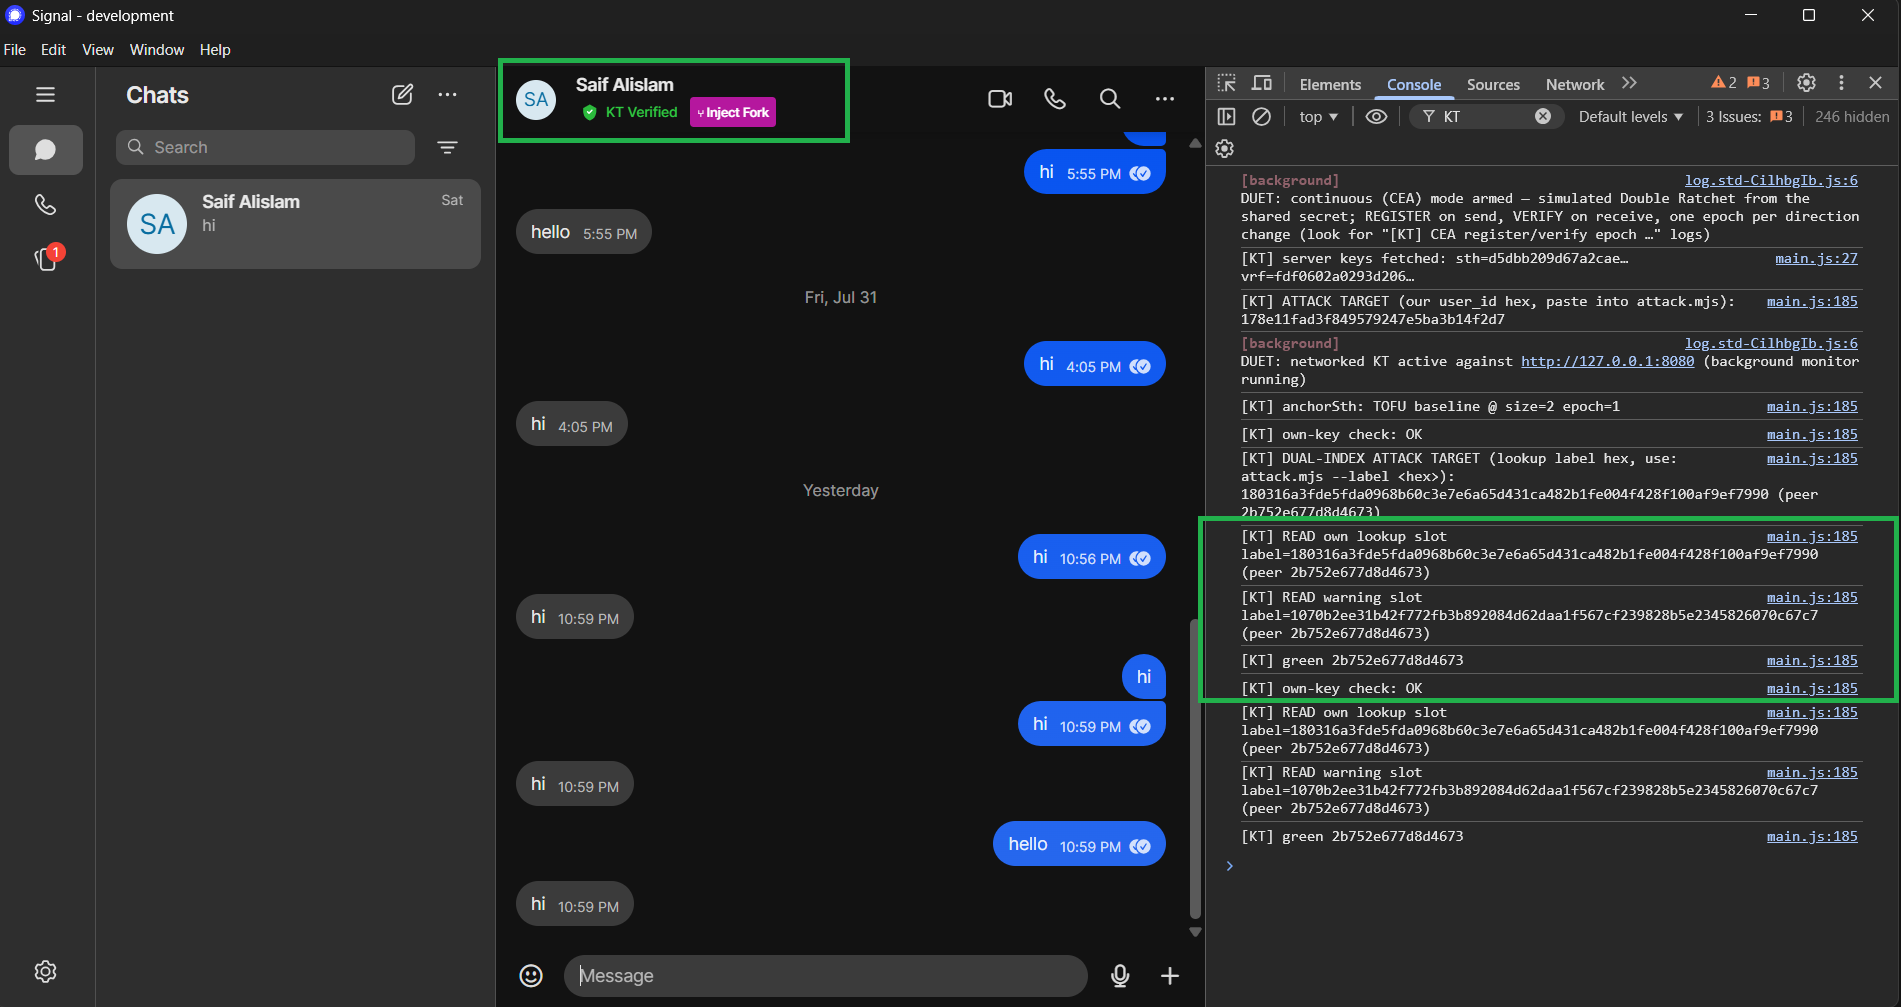
\includegraphics[width=\textwidth]{figures/normal.png}
\caption[Verified state before an attack.]{The client displays a verified state after successful
owner- and warning-slot checks.}
\label{fig:impl-baseline}
\end{figure}

\begin{figure}[p]
\centering
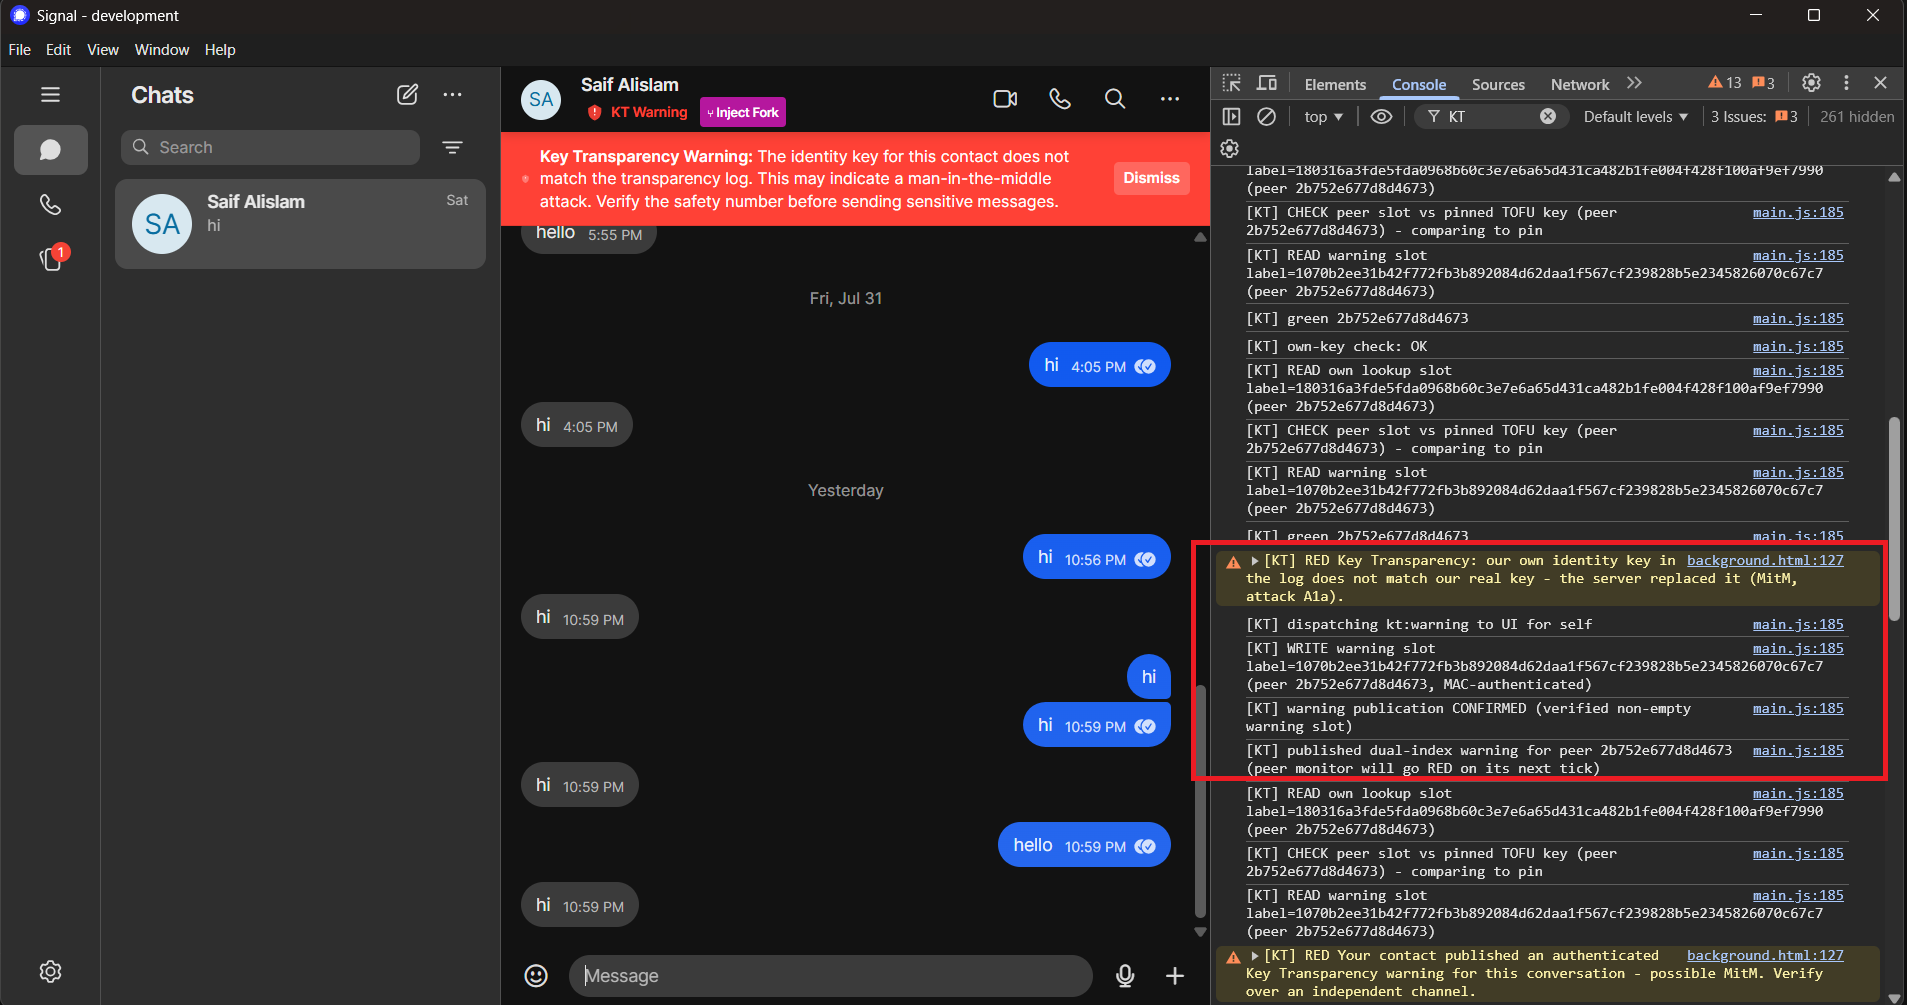
\includegraphics[width=\textwidth]{figures/attacked_user.png}\\[8pt]
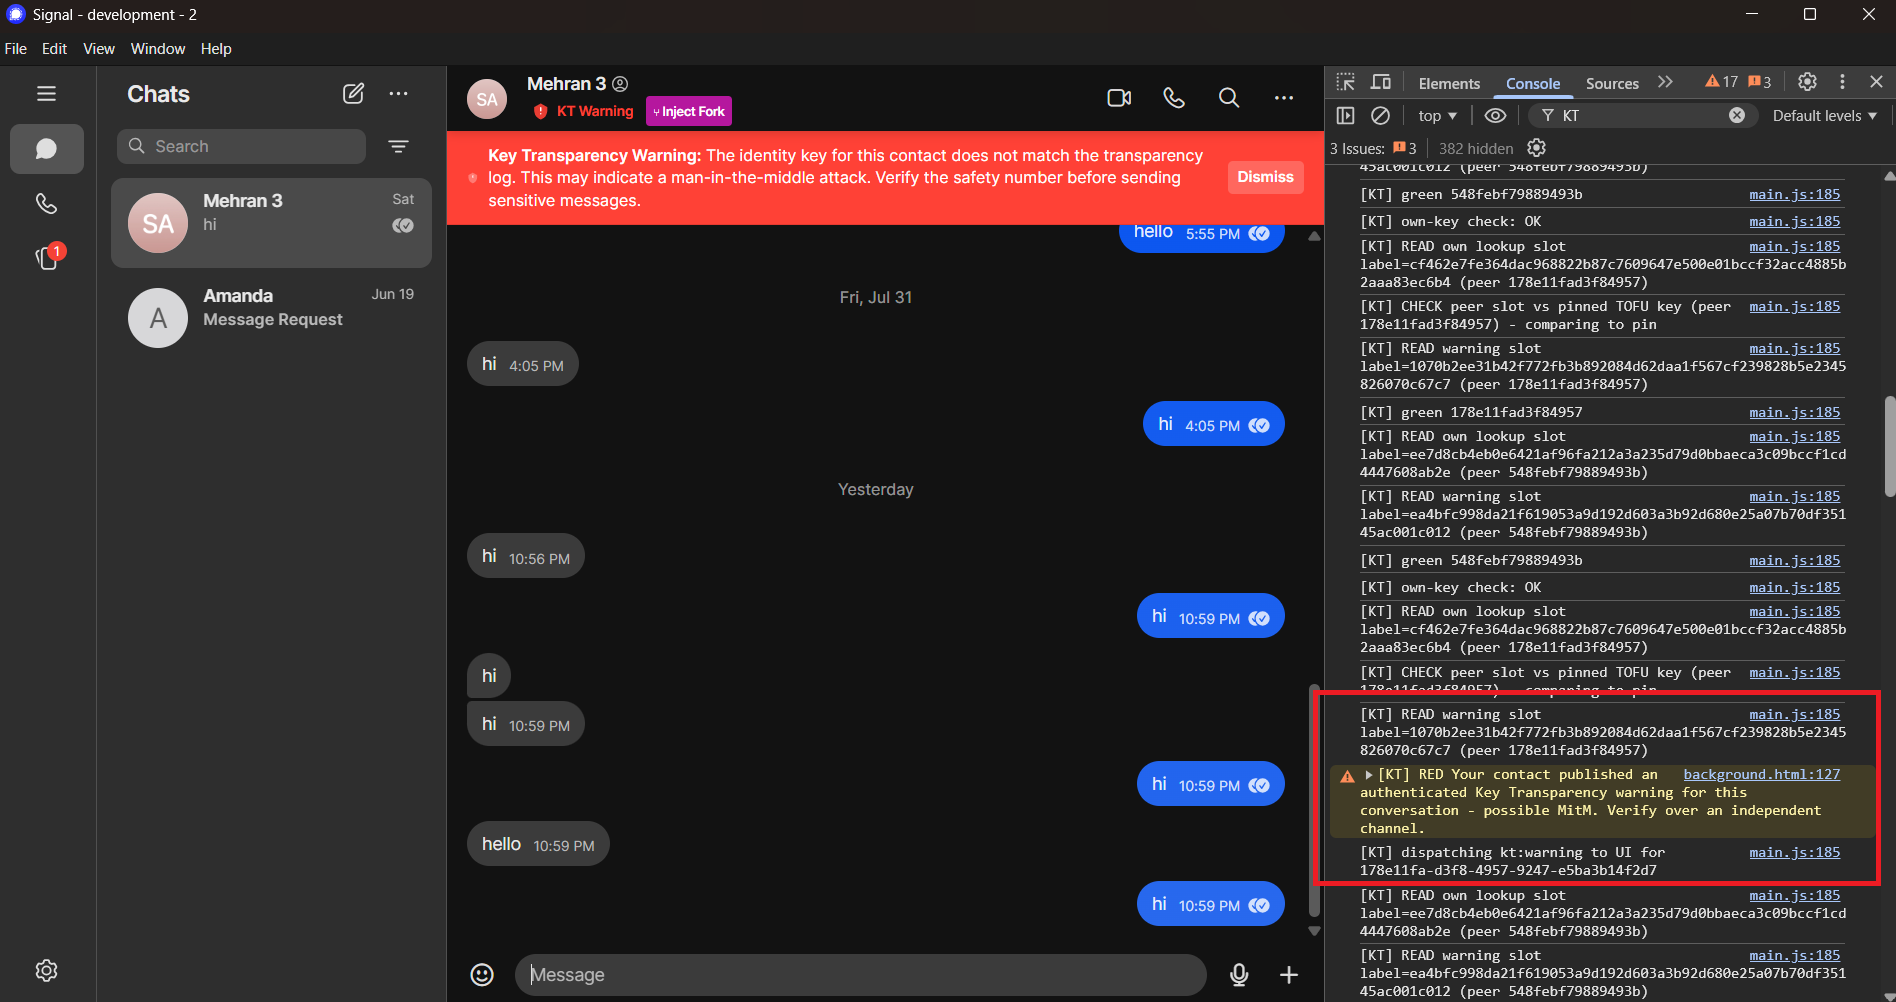
\includegraphics[width=\textwidth]{figures/peer.png}
\caption[Identity-slot warning on both clients (A1a).]{The affected client detects the substituted
identity key and publishes a warning. The peer verifies the shared warning, and both clients display
the red banner.}
\label{fig:impl-screens}
\end{figure}

% ============================================================================
\FloatBarrier
\section{Cross-Implementation Testing and Parity}\label{sec:impl-tests}

Testing connects the two implementations and the security claims. RFC vectors check the ECVRF. Fixed
cross-language vectors require byte-for-byte agreement for label derivation, warning payloads, and CEA
evolution. A live wire-parity suite checks the TypeScript verifier against signed heads, VRF outputs,
Merkle proofs, and consistency proofs produced by the Rust directory server. The Rust integration and
cryptographic suites run against a real in-process \texttt{KTServer} rather than a mock, and the
adversarial suite at \texttt{tests/adversarial.rs} covers A0,
\hyperref[sc:threat-a1]{A1a and A1b}, \hyperref[sc:threat-a2]{A2},
\hyperref[sc:threat-a3]{A3}, \hyperref[sc:threat-a4]{A4},
\hyperref[sc:threat-a5]{A5}, and \hyperref[sc:threat-x1]{X1}. These tests
establish agreement and expected behaviour for the specified inputs, not equivalence over every input.
The complete counts, names, and outcomes are in \cref{sec:tests-evidence}, within \cref{app:tests}.

The Rust tests exhaustively cover every Merkle-log
inclusion proof and every consistency pair up to size 64, together with forged-proof rejection, so the
log implementation is checked against its full input space at that size rather than at sampled points.
The auditor is tested for a soundness pair as well as a liveness one. A genuine equivocation is
reported as \textsc{Fork}, while a divergent head carrying an invalid signature is rejected outright
rather than misclassified as a fork.

The TypeScript harness contains 116 Jest tests, and sixteen further embedded tests run inside Signal
Desktop's own runner across four suites, exercising realistic account identifiers through the live
integration boundary. These totals are distinct from each other and from the opt-in live wire-parity
suite, and they must not be presented as one interchangeable figure.
\Cref{sec:impl-repro} records the complete reproduction commands and environment.

% ============================================================================
\FloatBarrier
\section{System-Wide Engineering Challenges}\label{sec:impl-challenges}

Three problems materially changed the implementation. First, the initial TypeScript label stand-in
could not agree with Rust's RFC~9381 ECVRF, because the two encode-to-curve steps differed. Both
clients were aligned on the ECVRF-EDWARDS25519-SHA512-TAI suite and checked against the published
vectors. Signed heads were also bound to each lookup response at this point, preventing a valid proof
from being paired with an unsigned or unrelated head.

Second, registration and lookup originally encoded Signal account identifiers differently. Converting
the service-ID string once at the integration boundary gives both paths the same canonical 16-byte
input and excludes phone-number identifiers before processing. Concurrent registration separately
exposed a time-of-check race between reading the head and using it to bound a proof. Binding each
consistency proof to the already validated head size prevents a later commit from making the client or
auditor compare a proof against the wrong upper bound.

Third, Electron bundling and context isolation prevented reliable loading and delivery to the
interface, through three distinct obstacles. The bundler split the key-transparency code at its
dynamic imports, so the layer was kept in one bundle. Context isolation blocked assignments to
\texttt{window} while allowing DOM custom events to cross the preload and renderer boundary. The
application's typed event bus and those DOM custom events were then mismatched, which was resolved by
dispatching on both. The remaining bundling, deterministic-state, and reset detail is preserved in
\cref{sec:apiref-engineering}.

Within the uncompromised-endpoint assumption in \cref{sec:threat-assumptions}, directory-response
verification relies on the verifier, its cryptographic dependencies, the hand-written ECVRF, and the
operator's two public keys, which are fetched once at initialization. The verifier returns a rejecting
verdict for invalid or absent signed heads, incorrect roots, missing inclusion proofs, mismatching labels,
and invalid VRF bindings. Availability
failures produce an amber notice rather than a red integrity warning, so an unreachable directory server is
never reported as an attack. The Signal hook currently reports these verdicts but leaves
session-blocking policy to future work.

Deterministic seeded server keys, a genesis epoch, and an administrative reset make the demonstration
repeatable and prevent a failed operation on an empty log from leaving the shared state unusable. A
poisoned mutex is likewise survivable in the harness. Production handlers would still need explicit
recovery from lock failure rather than relying on demonstration setup.

% ============================================================================
\section{Reproducibility}\label{sec:impl-repro}

Reproducibility of the measurements in \cref{ch:eval} depends on a recorded environment and
deterministic cryptographic and sampling inputs. Fixed seeds determine the VRF key, label placement,
and sampled users. Each benchmark begins from fresh seeded server state, so no residual state carries
between runs, while the live demonstration uses the administrative reset. The Rust tests and
benchmarks are run with \texttt{cargo test} and \texttt{cargo bench}, respectively. The environment
record captures the hardware, operating system, compiler, and toolchain versions. The repository
layout and the one-command runner scripts are listed in \cref{sec:apiref-repo}.
